\section{Core Pressure, Confinement, and the Mechanical Origin of Mass and Time}

\subsection{Radial Pressure Field and Core Confinement}

The radial pressure profile around a vortex filament in the VAM follows:
\begin{equation}
    P(r) = \frac{1}{2} \rho_{\ae} \left( \frac{\Gamma}{2\pi r} \right)^2 = \frac{\rho_{\ae} \Gamma^2}{8\pi^2 r^2}
\end{equation}
To avoid singularity at \( r = 0 \), we introduce a core radius \( r_c \), below which the swirl transitions to solid-body rotation. At this boundary, maximum pressure reaches:
\begin{equation}
    P_{\text{max}} = \frac{1}{2} \rho_{\ae} C_e^2 \approx 2.3 \, \text{GPa}
\end{equation}

\subsection{Mass from Swirl Confinement}\label{subsec:mass-from-swirl}

A stable vortex excitation possesses inertial mass due to energy stored in confined swirl:
\begin{equation}
    m_f = \frac{\rho_{\ae} \Gamma^2}{3\pi r_c c^2}
\end{equation}
This mass arises mechanically from:
\begin{itemize}
    \item Vortex circulation \( \Gamma \),
    \item Core scale \( r_c \),
    \item Æther density \( \rho_{\ae} \).
\end{itemize}
Unlike the Standard Model, no Higgs field or symmetry breaking is needed; mass results from swirl confinement.

\subsection{Smoothed Core Profile}

To maintain physical continuity at the core, we define:
\begin{equation}
    v_\theta(r) =
    \begin{cases}
        \frac{\Gamma r}{2\pi r_c^2}, & r \leq r_c \\
        \frac{\Gamma}{2\pi r}, & r > r_c
    \end{cases}
    \qquad
    P(r) =
    \begin{cases}
        \frac{\rho_{\ae} \Gamma^2 r^2}{8\pi^2 r_c^4}, & r \leq r_c \\
        \frac{\rho_{\ae} \Gamma^2}{8\pi^2 r^2}, & r > r_c
    \end{cases}
\end{equation}

\subsection{Boundary Layers and the Bohr Radius}

As pressure decays outward, equilibrium with the background æther sets in around:
\begin{equation}
    R_{\text{eq}} \sim a_0 = \frac{4\pi \varepsilon_0 \hbar^2}{m_e e^2} \approx 5.29 \times 10^{-11} \, \text{m}
\end{equation}
This alignment with the Bohr radius suggests that atomic boundaries are not quantum abstractions but hydrodynamic equilibrium shells.

\subsection{Ætheric Time Dilation}

Building on the helicity model from Section XII, we compute the explicit time dilation:
\begin{equation}
    \frac{d\tau}{dt} = \sqrt{1 - \frac{v_\theta^2}{c^2}} \approx 1 - \frac{P(r)}{\rho_{\ae} c^2}
\end{equation}
At the core, where \( P \approx P_{\text{max}} \), this yields:
\begin{equation}
    \frac{d\tau}{dt} \approx 1 - \left(\frac{C_e}{c}\right)^2 \approx 1 - 6.5 \times 10^{-10}
\end{equation}
This confirms that \emph{inertial time dilation} arises from centrifugal swirl pressure in the æther, independent of relativistic or gravitational sources.

\begin{figure}[H]
    \centering
    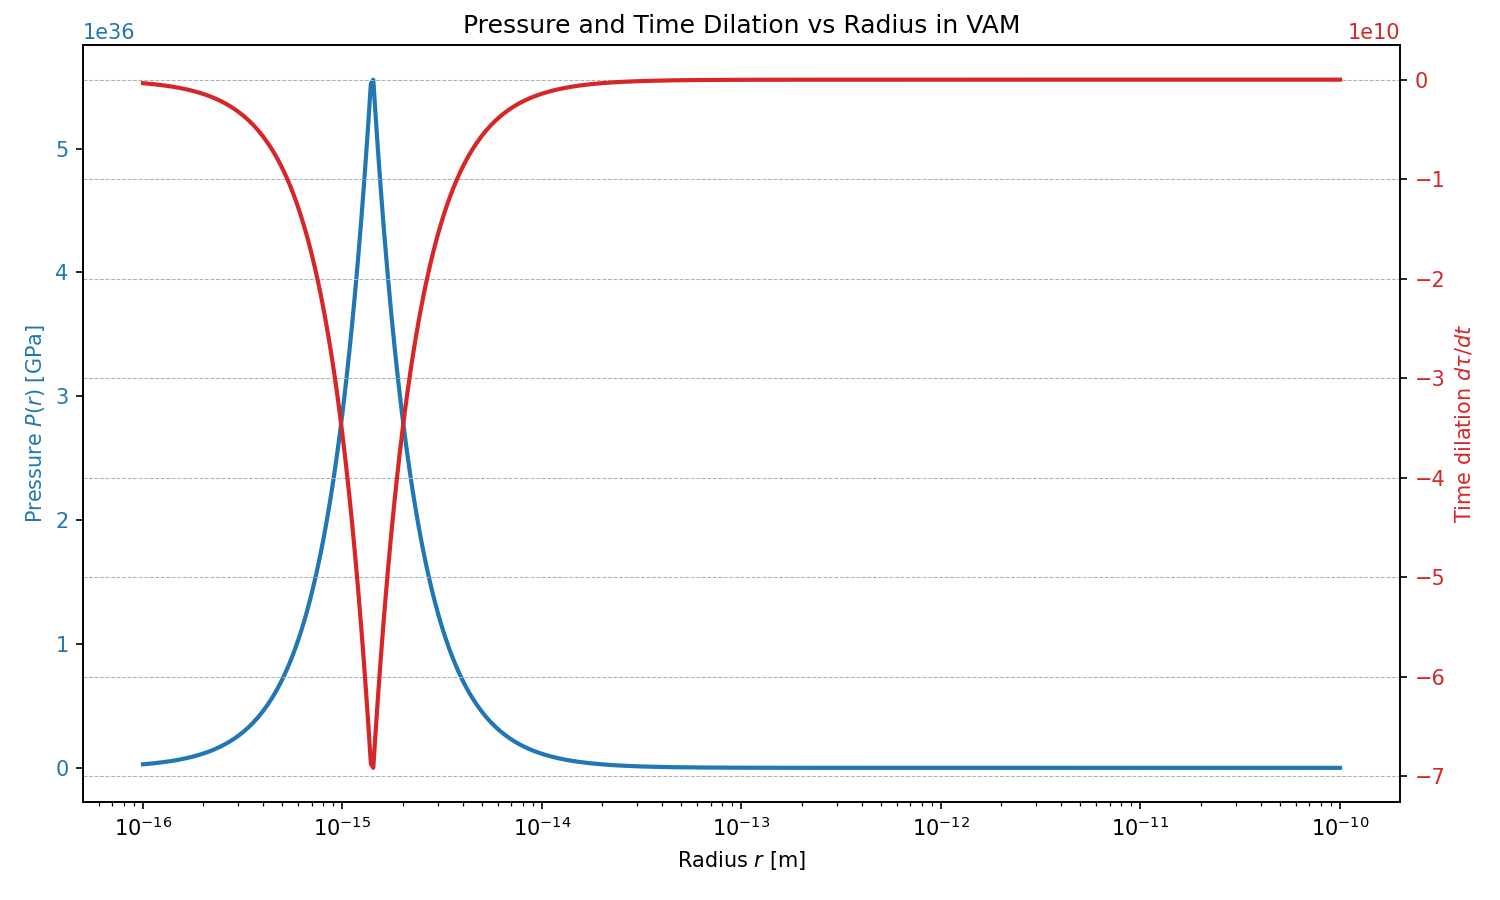
\includegraphics[width=0.85\textwidth]{images/TimeDilationCore}
    \caption{%
        \textbf{Radial profile of swirl-induced pressure and time dilation in the Vortex Æther Model (VAM).}
        The pressure field (blue) peaks near the core radius \( r_c \sim 10^{-15} \,\mathrm{m} \), inducing time dilation (red) via inertial swirl stress. Local clock rates slow subtly in high-pressure regions, consistent with helicity-based temporal emergence. This mechanism provides a fluid-mechanical origin for time dilation without invoking relativistic motion or curvature.
    }
    \label{fig:time_dilation_profile}
\end{figure}

\subsection{Mechanical Ontology Summary}

\begin{table}[H]
    \centering
    \begin{tabular}{|l|l|l|}
        \hline
        \textbf{Feature} & \textbf{VAM Interpretation} & \textbf{Standard Model Analogy} \\
        \hline
        Core Pressure Spike & Swirl-based confinement & QCD bag pressure \\
        Mass & Ætheric swirl inertia & Higgs-generated rest mass \\
        Boundary Layer \( R_{\text{eq}} \) & Swirl equilibrium zone & Bohr radius \\
        Time Dilation & Ætheric stress response & Relativistic redshift \\
        Inertia & Resistance to vortex deformation & Undefined in QFT \\
        \hline
    \end{tabular}
    \caption{Comparison of physical mechanisms in VAM and the Standard Model.}
\end{table}

\subsection*{Final Implication}

The 2.3–2.5GPa pressure spike embodies the ætheric stress needed to stabilize vortex matter and locally warp temporal flow. These structures encode mass, inertia, and clock rate without invoking fields, curvature, or postulates—offering a purely mechanical account of quantum phenomena.

\subsection{Knotted Vortex Molecules and Swirl-Mediated Binding}

Recent work on black hole binaries and scalar/vector fields has shown that compact astrophysical objects can form quasi-stable composite structures, termed ``gravitational molecules'' \cite{baumann2023black}. These emerge from resonant coupling between the orbiting black holes and bound modes of a surrounding field.

In the Vortex Æther Model (VAM), we propose an analogous mechanism: \textit{knotted vortex molecules}. These are topologically stable vortex bundles whose mutual interactions are mediated by the exchange of long-range swirl modes — low-energy excitations in the surrounding fluid æther.

\subsubsection*{Swirl-Mediated Binding Potential}

Let $|K_1\rangle$ and $|K_2\rangle$ be two knotted vortex states characterized by twist $T_i$, chirality $C_i$, and linking $Lk_i$. The effective potential between them is determined by:
\begin{equation}
V_{\text{int}}(r, \Delta T, \Delta C) \sim -\frac{\Gamma^2}{r^n} \cos(\omega_{\text{res}} t)
\end{equation}
where:
\begin{itemize}
    \item $\Gamma$: circulation strength of each vortex,
    \item $r$: separation distance,
    \item $\omega_{\text{res}}$: natural resonance frequency set by relative swirl twist and chirality,
    \item $n = 1, 2, 3$: decay exponent based on swirl field dimensionality.
\end{itemize}

\subsubsection*{Bound Swirl States and Resonant Modes}

When $\omega_{\text{res}}$ matches a standing wave mode of the inter-vortex field, the two knots may enter a stable resonant configuration. These states obey discrete spectrum conditions:
\[
\omega_n \sim \frac{2\pi n}{L_{\text{eff}}}
\quad \text{with } n \in \mathbb{Z}
\]
where $L_{\text{eff}}$ is the characteristic length of the connecting swirl tube.

Such bound states are **analogous to vibrational modes** in molecular physics or atomic orbitals, and may explain mass hierarchies or flavor oscillations.

\subsubsection*{Topological Interpretation of Molecular States}

Each vortex molecule is characterized by:
\begin{itemize}
    \item An effective topological quantum number: $Q = \text{Link}(K_1, K_2)$,
    \item A composite twist: $T_{\text{tot}} = T_1 + T_2 + T_{\text{exchange}}$,
    \item A dynamical chirality coupling: $C_{\text{eff}} = C_1 \cdot C_2$.
\end{itemize}

The energy levels of such configurations may be derived from topological invariants or spectral analysis of the swirl field Laplacian:
\[
\mathcal{L}_{\text{swirl}} \phi = \omega^2 \phi, \quad \text{subject to knotted boundary conditions}
\]

\subsubsection*{Confinement and Stability}

Analogous to color confinement in QCD, isolated vortex knots with certain quantum numbers (e.g. non-zero $Q$ or $C$) may not be stable unless part of a molecular state. The formation of bound triskelion or tetra-knot structures could thus model baryons, mesons, or exotic hadrons within a topological fluid context.

